El aprendizaje autom\'atico es una rama de la inteligencia artificial que tiene como objetivo el desarrollo de algoritmos que permitan a la m\'aquina aprender de la experiencia. \\

Este trabajo tiene como objetivo mejorar la medida del momento transverso de muones de alto-$p_{T}$. Puesto que CMS dispone de simulaciones precisas sobre la producci\'on, propagaci\'on y proceso de medida de dichos muones, en donde el momento real de la part\'icula es conocido, este trabajo se centrar\'a en un m\'etodo supervisado. De esta forma, al modelo matem\'atico se le proporcionan, en la fase de aprendizaje o entrenamiento, tanto las caracter\'isticas del mu\'on (datos de entrada), como el momento transverso real asignado en la simulaci\'on de la part\'icula, con el fin de que en esta etapa el modelo pueda encontrar correlaciones y patrones de comportamiento en los datos de entrada que mejoren la estimaci\'on del $p_{T}$ del mu\'on. Posteriormente, en el proceso de testeo, el modelo ha de ser capaz de dar una predicci\'on del $p_{T}$ tomando como datos de entrada de muones con momento transverso desconocido. \\

Dentro de los distintos tipos de algoritmos de aprendizaje autom\'atico destacan las redes neuronales artificiales, cuyo funcionamiento se inspira en la redes neuronales biol\'ogicas que forman el cerebro, y se componen de unidades conectadas denominadas neuronas que reciben una cierta informaci\'on, la procesan, y la transmiten a las siguientes neuronas con las que est\'an conectadas. La estructura esquem\'atica de una red neuronal se muestra en la Figura~\ref{fig:ann}, y est\'a formada esencialmente por capas de neuronas conectadas entre s\'i, donde cada conexi\'on lleva asociado un peso que da cuenta de la importancia que tiene la informaci\'on que va de una neurona a otra. \\

\begin{figure}[h]
\centering
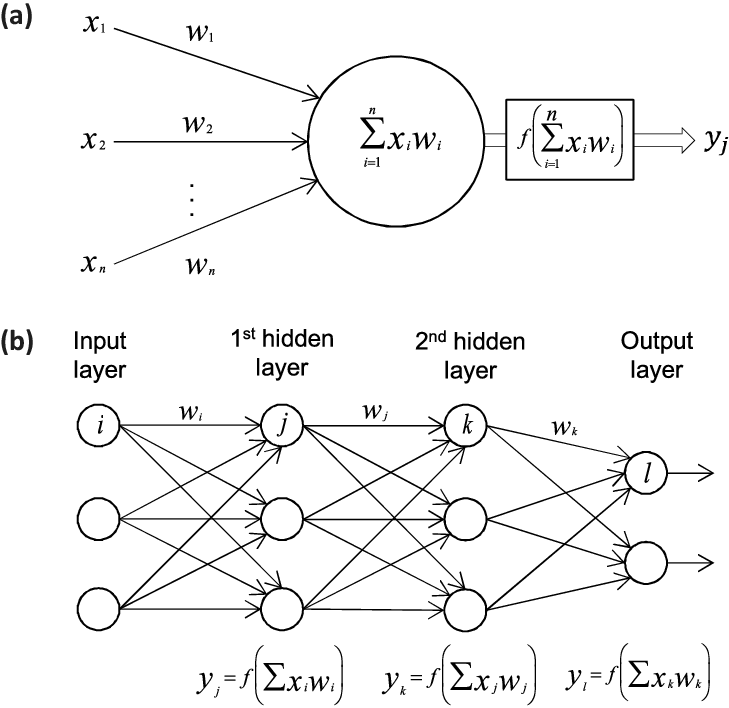
\includegraphics[width=0.70\textwidth]{figures/a-The-building-block-of-deep-neural-networks-artificial-neuron-or-node-Each-input-x.png}
\caption{Representaci\'on gr\'afica del funcionamiento de una red neuronal artificial. a: procesamiento de una neurona, donde cada entrada $x_{i}$ lleva asociado un peso $w_{i}$, y la suma de todas las entradas pesadas que llega a la neurona se pasa a la siguiente neurona tras aplicar una funci\'on de activaci\'on no lineal. b: ejemplo de una red neuronal multicapa donde las neuronas de cada capa est\'an conectadas a todas las neuronas de la capa siguiente. La informaci\'on es propagada desde la primera capa hasta la capa final, donde se eval\'ua el error en la predicci\'on. Imagen tomada de \cite{Vieira2017}.}
\label{fig:ann}
\end{figure}

El proceso de transmisi\'on de informaci\'on va de izquierda a derecha: en primer lugar se inicializan los pesos de la red (habitualmente de manera aleatoria) y se tiene una primera capa de neuronas que se corresponden con las distintas variables de entrada. Si todas las neuronas de una capa est\'an conectadas con las neuronas de la capa siguiente, a cada neurona de la siguiente capa le llegar\'a como entrada un sumatorio de la informaci\'on de cada neurona de la capa anterior multiplicada por su peso asociado, de manera que a esta entrada se le aplica una funci\'on de activaci\'on no lineal y se sigue propagando la informaci\'on a las siguientes capas. \\
Una vez que la informaci\'on llega a la capa final de la red, se eval\'ua el error en la predicci\'on respecto al valor real conocido de la magnitud que se quiere predecir. \\

Por otra parte, el proceso de aprendizaje a partir de la experiencia se hace en la direcci\'on contraria: una vez obtenido el error en la predicci\'on, los pesos se van actualizando capa a capa hacia atr\'as acorde a la direcci\'on del gradiente de la funci\'on de error, de forma que se busca que en la siguiente iteraci\'on el error en la predicci\'on sea menor. \\

La red neuronal profunda o DNN se distingue de la red neuronal convencional por tener m\'as capas ocultas y un mayor n\'umero de neuronas en cada capa, aumentando as\'i la cantidad de par\'ametros, nivel de abstracci\'on y complejidad, y permitiendo obtener un mayor rendimiento en la predicci\'on para conjuntos de datos de entrada de gran dimensionalidad. \\

En f\'isica de altas energ\'ias, el uso de las redes neuronales profundas se ha extendido en los \'ultimos a\~nos, siendo una de las herramientas m\'as utilizadas en la reconstrucci\'on de objetos f\'isicos y en la clasificaci\'on de eventos en b\'usquedas de nuevas part\'iculas (ver \cite{collaboration2020IdentificationOH}). 
